\chapter{SPRINT TWO - Communication and sales}
\minitoc
\newpage
\section*{Introduction}
\addcontentsline{toc}{section}{Introduction}
In this sprint, we will be developing the part where the instructor will communicate with the students and manage the sales.
\section{Sprint backlog}
%%%%%table
\begin{table}[H]
\centering
\caption{Product backlog}
\begin{tabular}{|p{1cm}|p{3cm}|p{6cm}|p{2cm}|}
\hline
\rowcolor{brown!18}\textbf{\large{ID}} & \textbf{\large{As a}} & \textbf{\large{I want to be able to}} & \textbf{\large{Priority}} \\
\hline
5& Instructor & Send messages to my students & High\\\hline
6& Instructor & Recieve messages from my students  & High\\\hline
7& Instructor  & See my course sales & Normal \\\hline
\end{tabular}
\end{table}
%%%%%table
\section{Requirement analysis}
\subsection{Use case diagram}

\begin{figure}[!ht]
    \centering
    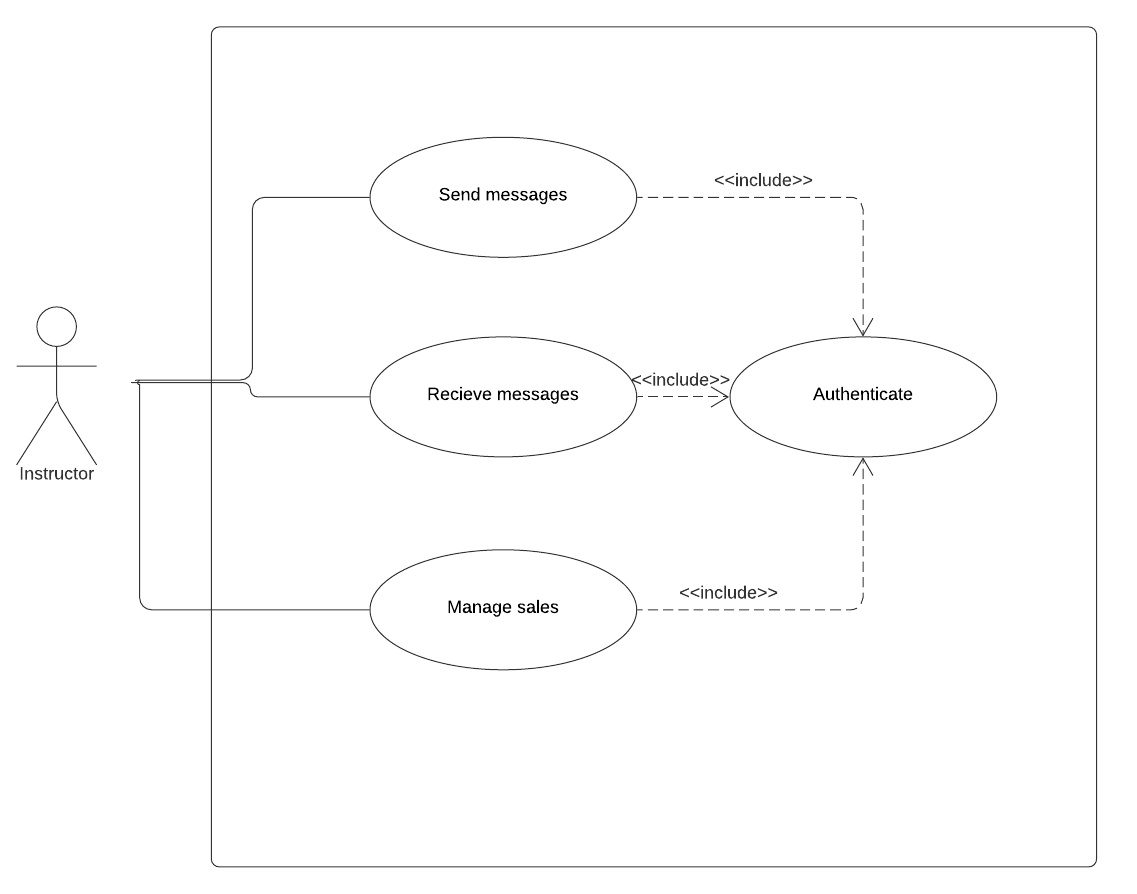
\includegraphics[width=120mm]{sprint2usecase.png}
    \caption{Sprint 2 use case diagram}
    \label{fig:sprint2usecase}
\end{figure}




\subsection{Modeling}

%%%%%table
\begin{table}[H]
\centering
\caption{send messages textual description}
\begin{tabular}{|p{4cm}|p{10cm}|}
\hline
\textbf{\large{Use case name}} & Send messages \\\hline
\textbf{\large{Actors}} & Instructor \\\hline
\textbf{\large{Preconditions}} & User logged in \\\hline
\textbf{\large{Postconditions}} & Message sent  \\\hline
\textbf{\large{Normal flow}} & 
\begin{itemize}
  \item The instructor visits the instructor space.
  \item The instructor clicks the communication tab.
  \item The instructor opens the conversation.
  \item The instructor type the message and clicks send.
\end{itemize}
\\\hline

\end{tabular}
\end{table}
%%%%%table

\begin{figure}[!ht]
    \centering
    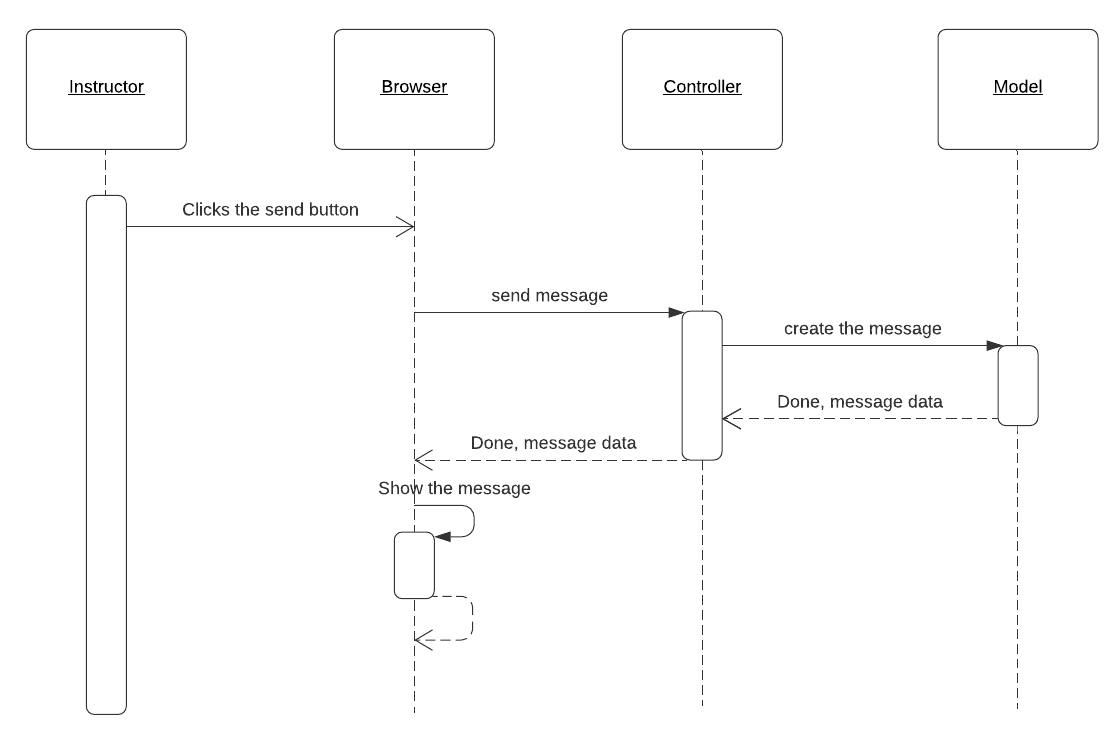
\includegraphics[width=142mm]{seq_send_message.png}
    \caption{Sequence diagram of sending a message}
    \label{fig:seq_send_message}
\end{figure}

%%%%%table
\begin{table}[H]
\centering
\caption{recieve messages textual description}
\begin{tabular}{|p{4cm}|p{10cm}|}
\hline
\textbf{\large{Use case name}} & Recieve messages \\\hline
\textbf{\large{Actors}} & Instructor \\\hline
\textbf{\large{Preconditions}} & User logged in \\\hline
\textbf{\large{Postconditions}} & Message recieved and seen \\\hline
\textbf{\large{Normal flow}} & 
\begin{itemize}
  \item The instructor visits the instructor space.
  \item The instructor clicks the communication tab.
  \item The instructor opens the conversation.
  \item The instructor type sees the messages recieved.
\end{itemize}
\\\hline

\end{tabular}
\end{table}
%%%%%table

\begin{figure}[!ht]
    \centering
    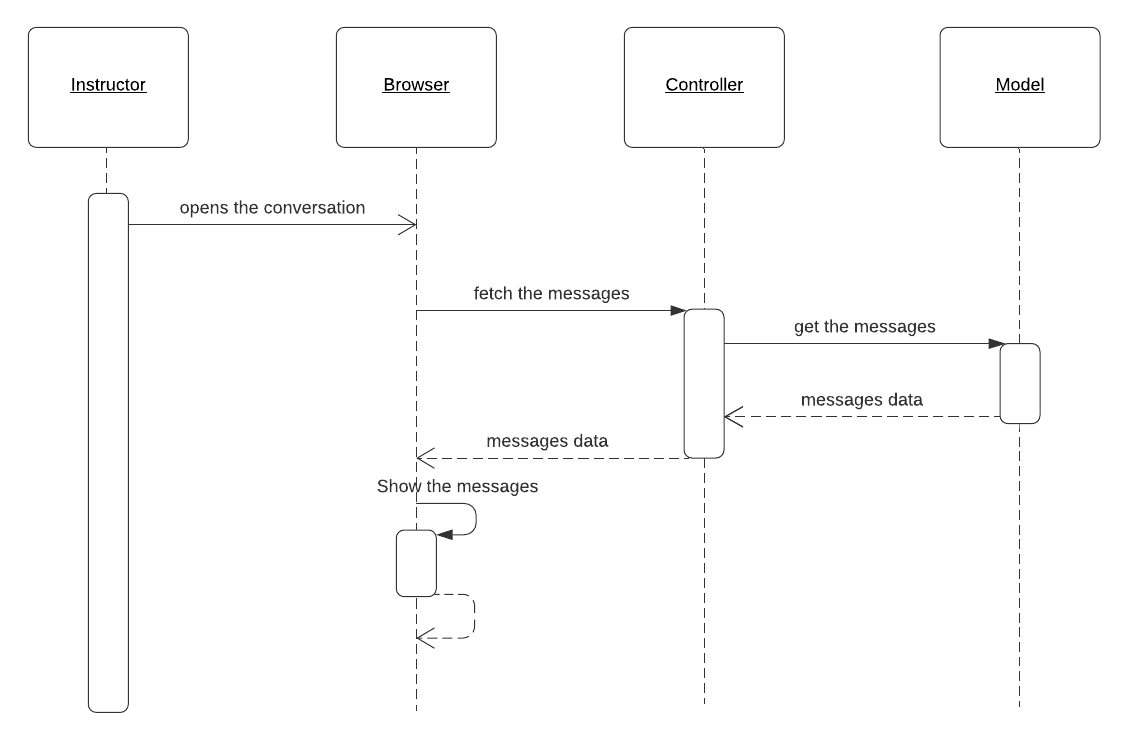
\includegraphics[width=150mm]{seq_recieve_message.png}
    \caption{Sequence diagram of recieving a message}
    \label{fig:seq_recieve_message}
\end{figure}

%%%%%table
\begin{table}[H]
\centering
\caption{manage sales textual description}
\begin{tabular}{|p{4cm}|p{10cm}|}
\hline
\textbf{\large{Use case name}} & Manage sales \\\hline
\textbf{\large{Actors}} & Instructor \\\hline
\textbf{\large{Preconditions}} & User logged in \\\hline
\textbf{\large{Postconditions}} & Sales managed  \\\hline
\textbf{\large{Normal flow}} & 
\begin{itemize}
  \item The instructor visits the instructor space.
  \item The instructor clicks the performance tab.
  \item The instructor sees statistics about their sales and earnings.
\end{itemize}
\\\hline

\end{tabular}
\end{table}
%%%%%table


\begin{figure}[!ht]
    \centering
    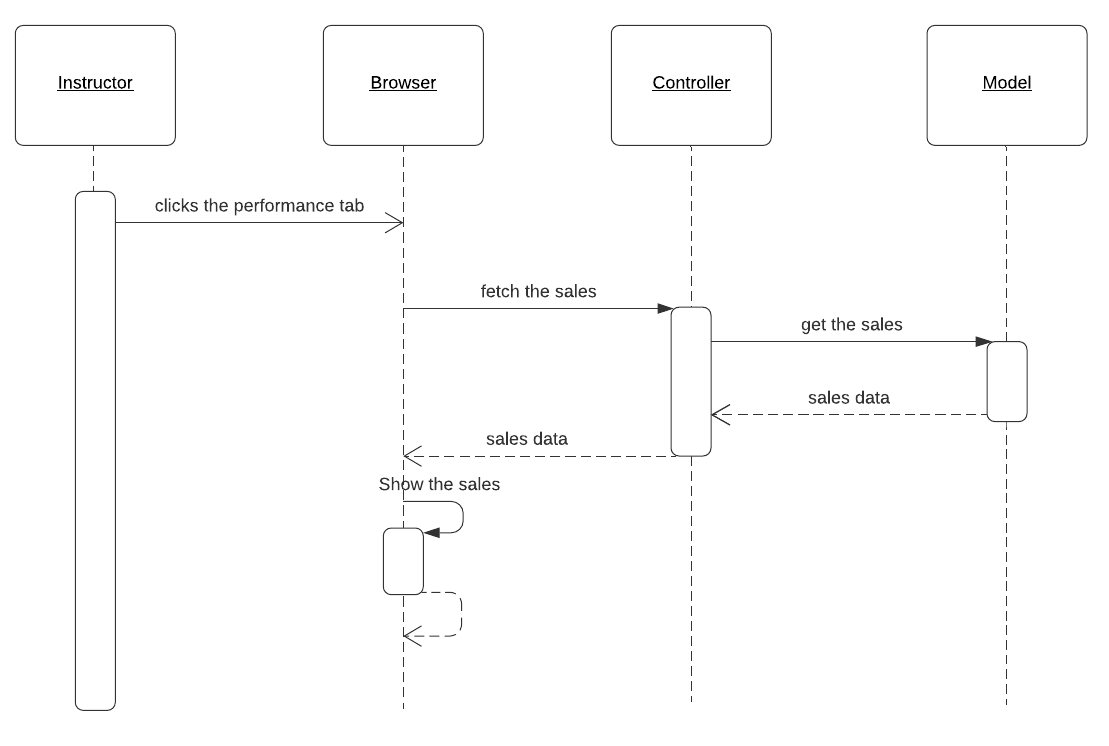
\includegraphics[width=150mm]{seq_sales.png}
    \caption{Sequence diagram of visitng sales}
    \label{fig:seq_sales}
\end{figure}


\section{Implementation}


\subsection{Sending a message}
When clicking on the send button, we send the message written to the server and in return we get the created record in the database. We add the result to the redux messages reducer to update the interface and show the sent message.

\subsection{Recieving messages}
Upon opening a conversation, the browser will make a request to the server to fetch the message of that conversation and show it to the user.
\hfill \break
Since we are not building a chat app, we avoided using realtime solutions like sockets to fetch messages without refreshing the page as it will cause more load on the server. So we chose to do long polling :  pick a random timer in a specific range and each time that timer expires we make a request to the server looking for new messages and show them to the user. 

\begin{figure}[!ht]
    \centering
    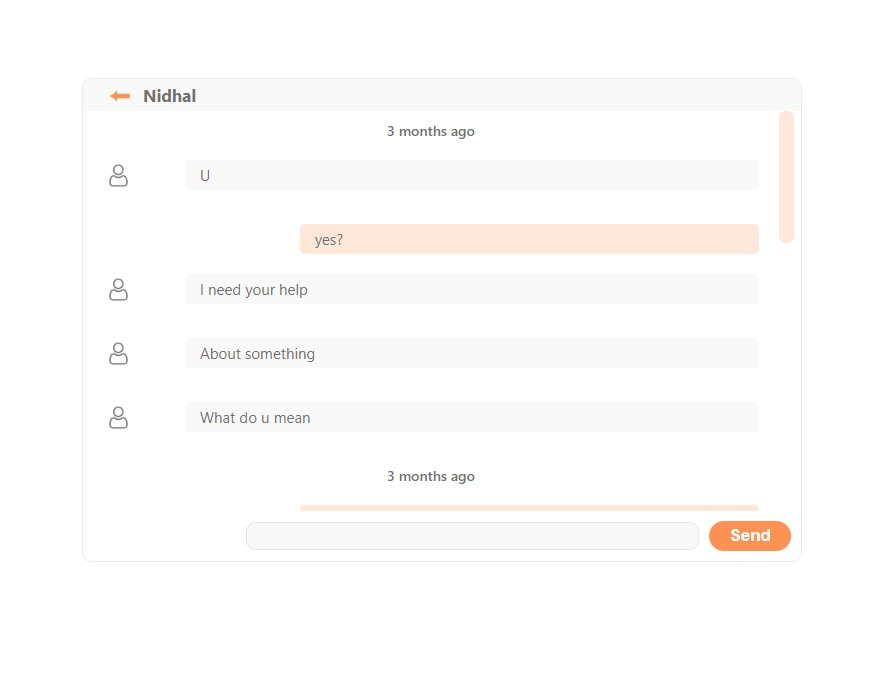
\includegraphics[width=150mm]{conversation2.jpg}
    \caption{Conversation interface}
    \label{fig:conversation2}
\end{figure}

\subsection{Manage Sales}
Clicking on the performance tab will bring up a page where the instructor see statistics about their sales and earnings. Upon visiting this page, the browser will make a request to the server to fetch all the necessary data and show them to the user.
\hfill \break
\hfill \break
We used react-chartjs-2 library to show the earnings of each month for the user in a graph. 
\hfill \break
\hfill \break
We also used react-data-table-component library to show the sales data in a table, this library helps us with sorting the data by a specific colum. The sorting happens in the server, so each time the user chose to sort by certain colum, we send a request to the server with the colum that we want to sort on, get the data and show it to the user accordingly. The library also helps us with the server side pagination, so that each time the user request a specific page we send a request to the server with the page number and fetch the data. 

\hfill \break
\hfill \break

\begin{figure}[!ht]
    \centering
    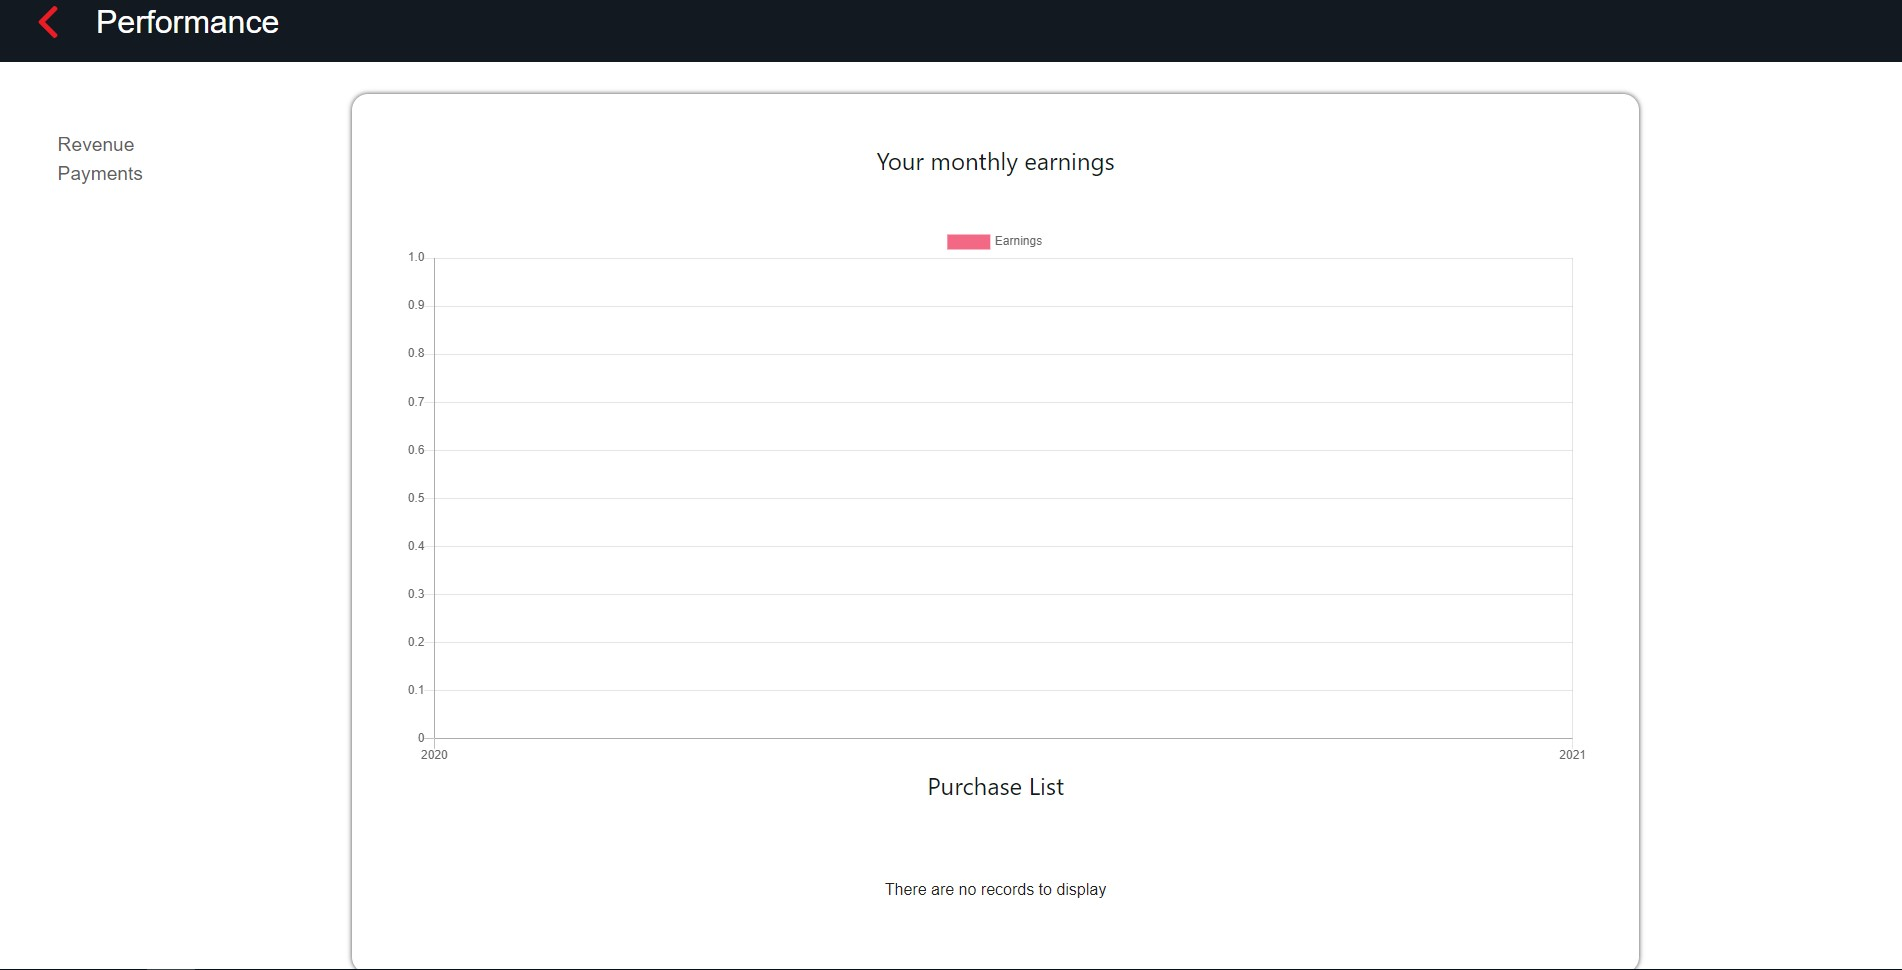
\includegraphics[width=150mm]{earnings.jpg}
    \caption{Sales page interface}
    \label{fig:earnings}
\end{figure}


\vfill
\clearpage

\section*{Conclusion}
In this chapter, we coved the communication part of the app and how the instructor can manage his sales.
\addcontentsline{toc}{section}{Conclusion}